%%%%%%%%%%%%%%%%%%%%%%%%%%%%%%%%%%%%%%%%%%%%%%%%%%%%%%%%%%%%%%%%%%%%%%%%%%%%%%%%%%%%%%%%%%
%                       Document réalisé par Théo Vanden Driessche
%                               En novembre 2017 
%                    %dans le cadre du cours de géographie de 6A D CSM
%
%
%%%%%%%%%%%%%%%%%%%%%%%%%%%%%%%%%%%%%%%%%%%%%%%%%%%%%%%%%%%%%%%%%%%%%%%%%%%%%%%%%%%%%%%%%%

\documentclass{article}
\usepackage[utf8]{inputenc}

\title{Geschiedenis}
\author{vandendriesschetheo }
\date{November 2017}
\usepackage{graphicx}
\graphicspath{ {images/} }



\usepackage{geometry}
 \geometry{
 a4paper,
 total={170mm,257mm},
 left=20mm,
 top=20mm,
 }



\begin{document}

\maketitle

\section{Eerste wereld oorlog}
\subsection{De spanningen namen toe}
'De grote oorlog' - periode 1914-1918 - was het eerste conflict waarin heel Europa betrokken was sinds het einde van de napoleontische oorlogen een eeuw voordien. Hij werd vooral uitgevochten op he Europese Continent en werd pas wereldoorlog door de deelname van de VS en de weerslag in de koloniale wereld

\subsubsection{De naderende oorlog...}
\begin{enumerate}
    \item In Europa kwamen twee bonden tot stand:
    \begin{itemize}
        \item In 1882 kwam een driebond tot stand tussen: Duitsland, Italie en Oostenrijk-Hongarij.
        \item In 1907 kwam een tripel entente tot stand tussen: Frankrijk, Groot-britanie en Rusland.
        \item Opmerking: Vooral de spanningen tussen Frankrijk en Duitsland was heel groot in die periode! Bij de inmaking van Duitsland in 1871 werd Elzas-Lotharingen een Duitse gebied.
    \end{itemize} 
\end{enumerate}

\subsubsection{Gewapende vrede}
De periode voor de oorlog tusse 1880 en 1914, was niet rustig. Verschillende landen voerdden een imperialistische politiek: \\
De landen investeren meer en meer geld in militaire producten.

\subsubsection{28 juni 1914}
\begin{itemize}
    \item Wat gebeurde er op 28 juni 1914?\\
    Frans Ferdinand, hertoog van OH, werd doodgeschoten door een serbische nationalist in Sarajevo.(gestuurd door Rusland.)
    \item Waarom gebeurde deze aanslag?\\
    De servische nationalisten willen niet dat Bosnië een deel van de dubblemonarchie Oostenrijk-Hongarije komt.
\end{itemize}
\subsection{De eerste wereldoorlog (1914-1918)}
\begin{enumerate}
    \item Van 'Blitzkrieg tot loopgravenoorlog. 
    \begin{itemize}
        \item Wat is dè Blitzkrieg?\\
        De duitser slaagt erin om heel snel Parijs te berijken door Belgie over te stekken.(de Van Schlieffenplan)
        \item Wat is de 'loopgravenoorlog'?\\
        Een trage en vuile oorlog.
    \end{itemize}
    \item Het beslissende jaar 1917.
    \begin{enumerate}
        \item Amerika.
        \newline
        \newline
        Vanaf 6 april 1917 namen de Verenigde Staten deel aan de oorlog. Aan het begin hadden de Amerikanen geen zin om deel te nemen aan de oorlog? Dit kwam onder andere door de Monroedoctrine.
        \begin{itemize}
            \item De Monroedoctrine:\\
            Een idée/beginsel van de Amerikaanse politiek van de 19De eeuw omleent aan J. Monroe in 1823. America moet met zijn eigen politieke problemen bezig houden.
        \end{itemize}
        Onder meer tengevolge van de duikbotenoorlog (1917) probeerde de Amerikaanse president Wilson de publieke opinie te veranderen. Dit lukte.\\
        \newline
        Woodrow Wilson (28 december 1856-3 februari 1924) was lid van de Democratische partij. Hij was 2 ambtersmijnen president.\\
        \item Rusland.
        \newline
        \newline
        De Russen verlieten het front in december 1917. Ten gevolge van de Russische Revolutie verlieten de Russen de oorlog. Dit werd vastgelegt in de Vrede Van Brest-Litovsk in maart 1918.\\
        \newline
        De bolsjevieken in Rusland sloten 'vrede' met de Centralen( Duitsland, Oostenrij-Hongarije, het Ottomaanse Rijk en Bulgarije).
    \end{enumerate}
    \item Het oorlogseinde (1918).\\
    Op 11 november 1918 werd in een treinwagon in het bos te Compiègne het Vredesverdrag ondertekend tussen Duitsland en de geallierden. Deze wapenstilstand wordt ieder jaar herdacht. Men herdenkt de slachtoffers van wereldoorlog I.
\end{enumerate}

\subsection{De gevolgen van de Eerste Wereldoorlog}
\begin{itemize}
    \item Er waren 10 miljoen slachtoffers waaronder ongeveer  1 miljoen burgers. Een hele generatie jongeren verdween.
    \item Verschillende steden werden vollefig verwoest waaronder historische steden zoals Antwerpen, Leuven en Ieper.
    \item Vele landen waren economisch uitgeput.
    \item Een blijvende vijandschap tussen Frankrijk en Duitsland.
\end{itemize}
\subsection{Het verdrag van Versailles}
\subsubsection{Uitgangspunten van de onderhandelaars.}

Vergadering van de leiders grootmacht: Frankrijk, Groot-Bratannië en de verenigde Staten in Versailles om het naoorloggse Europa vorm te geven.\\
Rond de tafel was er:
\begin{itemize}
    \item Woodrow Wilson, de VS president
    \item Georges Clemenceau, Franse Premier
    \item David Loyd, Britse permier
\end{itemize}
\begin{enumerate}
    \item De veertienpunten programma.\\
    President Wilson had een zeer idealistische porgramma om een sterke vrede te instellen.\\
    In zijn porgramma zat:
    \begin{itemize}
        \item Oprichting van de Volkenbond
        \item Zelfbeschikkingsrecht: onafhankelijkheid van landen 'vreemd bestuur'
        \item ontwapening
        \item afschaffen van militaire allianties.
    \end{itemize}
    \item Clemenceau en Lloyd.\\
    Maar de Europese leiders hadden minder idealistische bedoelingen. Ze hebben de oorlog aan de lijve meegemaakt en ze vresden nieuwe Duitse agressie.\\
    \begin{itemize}
        \item Economische en militair kortwieken.
        \item herstelbetalingen om de orloogsschade te compenseren
        \item bezetting van Duitse economische zones.
    \end{itemize}
    De Duitsen mochten niet deelnemen aan de onderhandelingen.
\end{enumerate}
\subsubsection{Het verdrag in praktijk: Europa hertekend.}
\begin{itemize}
    \item Oostenrijk-Hongaarse, Russische rijk en Duitse keizerrijk werd ontmanteld.
    \item Het Ottomaanse rijk werd ontmanteld. Ontstaan van Syrie en Irak.
    \item Onafhankelijke staten vinden plaats in van het gevallen Oostenrijk-Hongaarse en Russische rijk.bvb Esten, Lette, Polen, Hongarije
    \item Duitsland werd gezien als de aanstoker van de oorlog.
    \item Duitsland verloor geografische gebieden in het oosten en het westen. + zijn kolonies
    \item Duitse militaire gebied werd sterk gereduceerd en de vloot werd afgeschaft.
    \item Europese landen eisten heel hoge herstelbetalingen
    \item De droom van Wilson van een Volkenbond werd gerealiseerd. Deze instelling zou een neutrale 'internationale politieagent' worden 
    en zou de conflicten tussen de staten op een vreedzame manier zou kunnen oplossen.
    
\end{itemize}

\subsubsection{Reacties op het verdrag.}
\begin{itemize}
    \item Het verdrag van Versailles werd bij het Duitse politiek en het gewone volk negatief onthald. Het werd gezien als een Diktat.
    \item Duitsland kreeg ook een interne politieke crisis
    \item De Dolkstoot-mythe stelde dat het duitse volk deze problemen kende door een samenzwering van buitenlandse leiders, Duites politici en joden.
    \item De volkenbond kende een valse start. De Amerikaanse sennat steek het plan van Wilson weg.
    \item de Duitse ontevredenheid en de onmacht van de volkenbond zouden in de kommende decennia nog vaker voor problemen zorgen.
\end{itemize}

\subsubsection{De Europese gebieden die Duitsland verloor}
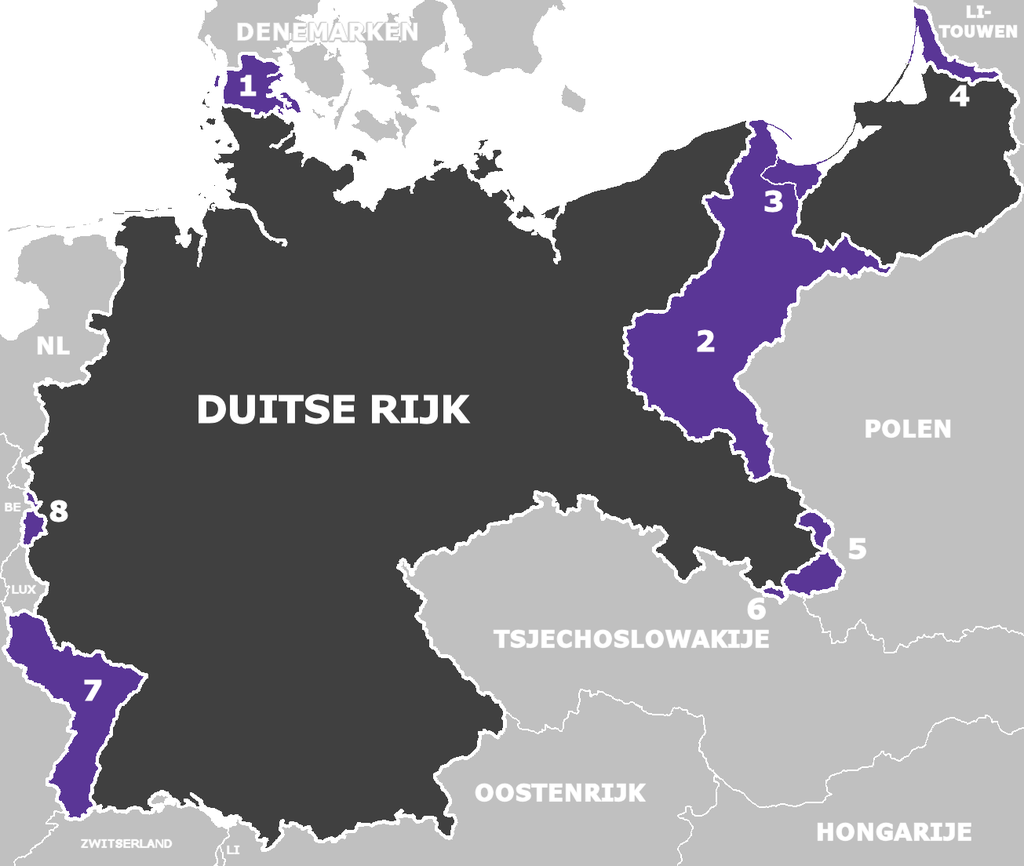
\includegraphics[scale=0.5]{DuitseRijk.png}
\begin{enumerate}
    \item Noord-Sleeswijk aan Denemarken
    \item Posen en West-Pruisen
    \item Vrije stad Dantzig
    \item Memel land aan Litouwen
    \item Oost-opper-Silezië aan Polen
    \item Hultschiner landje aan Tsjecho-Slovakije
    \item Elzas-Lotharingen aan Frankrijk
    \item Eupen-Malmedy aan België
\end{enumerate}

\newpage
\section{De Russische Revolutie}
\subsection{Inleiding}
\subsubsection{De Situatie voor 1917}
\begin{enumerate}
    \item Tsaar
    \begin{itemize}
        \item Tsaar Nicolaas II had alle macht in Rusland
        \item Tegenstanders werde opgepakt en naar Siberie verbannen (Geheime politie)
        \item Er kwam steeds meer kritiek op de tsaar.
    \end{itemize}
    \item Er was armoede in Rusland:
    \begin{itemize}
        \item De meeste mensen in Rusland leefden in armoed.
        \item De Communisten beloofden voor deze mensen op te zullen komen.
    \end{itemize}
    \item De figuur Raspoetin:
    \begin{itemize}
        \item De Eerste Wereldoorlog verliep voor Rusland dramatisch.
        \item Nicolaas stond aan het hoofd van het leger.
        \item De Tsaar stond onder invloed van Raspoetin(Een monnik met vreemde gewoonten).
    \end{itemize}
\end{enumerate}
\subsubsection{De revolutie begon}
\begin{enumerate}
    \item De straat op
    \begin{itemize}
        \item Er kwam steeds meer protest tegen de tsaar.
        \item Uiteindelijk gaf Tsaar Nicolaas II toe: Hij trad af. Er kwam een nieuwe regering (februari 1917).
    \end{itemize}
\end{enumerate}
\subsubsection{Lenin aan de macht}
\begin{enumerate}
    \item Lenin aan de macht
    \begin{itemize}
        \item De nieuwe regering kon de problemen niet oplossen.
        \item Op 25 oktober 1917 pleegde Lenin een staatsgreep.
    \end{itemize}
    \item Maatregelen van Lenin:
    \begin{itemize}
        \item Bedrijven in handen van de staat.
        \item Er kwam een nieuwe geheime politie.
        \item Vredesonderhandelingen met de Duitsers.
        \item gevolg: veel rijken vluchten het land uit.
    \end{itemize}
\end{enumerate}
\subsubsection{De man van staal}
\begin{itemize}
    \item In 1922 kreeg Rusland een andere naam: De Sovjet-Unie (USSR)
    \item Lenin stierf in 1924
    \item Opvolger is Jozef Stalin
\end{itemize}
\subsection{Revolte en revoluties in Rusland.}
\subsubsection{De revolte van 1905}
\begin{itemize}
    \item De tsaar regeerde op absolutistische manier in het agrarische Rusland. Liberalisering werd niet toegestaan.Mensen kwamen in opstand, vaak geïnspireerd door Karl Marx.
    \item In 1905 was er een revolutie.De burgerij, de arbeiders en soldate revolteren.Er kwam een nieuwe grondwet en een Doema voor de schijn. Dit revolte werd bloedig onderdrukt.
    \item De revolutionaire werden vervolgd. Op het heel platteland ontstaan revoltes, boeren namen het land van de aristocraten in bezit. Ze krijgen steun van de bolsjewieken(radicale revolutionnairen.)
\end{itemize}
\subsubsection{Mensjeviki en Bolsjeviki}
\begin{itemize}
    \item Mensjeviki:\\
    Trotski. De burgerije moet de leiding nemen.
    \item Bolsjeviki:\\
    Lenin,Stalin. Arbeiders en de boeren moet de leiding nemen.
\end{itemize}
\subsubsection{De februari revolutie van 1917}
\begin{itemize}
    \item De eerste Wereldoorlog bracht het revolutieproces op gang.
    \item In februari 1917 dit ongenoegen groeide tot een georganiseerd brood revolte in St Petersburg.
    \item Algemene stakingen en massale ongehoorzaamheid(ignorer les ordres) van arbeider en soldaten, die de sovjets vormden, dwongen de tsaar tot aftreden.
    \item De februari revolutie was een burgelijke revolutie.
    \item De grootgrondbezitters werd niet aangetast en de boeren kregen geen grond.
    \item De voorlopige regering voerde de oorlog verder. Voedselvoorziening ging beneden.
    \item Vele boeren hadden alle belang bij het succes van de Bolsjevieken.
    \item Er bestond 2 machtcentrums.
    \begin{itemize}
        \item De voorlopige regering stond onder leiding van de mensjevieken
        \item de Sovjets(raad): onder de leiding van de Boljsevieken.
    \end{itemize}
\end{itemize}
\subsubsection{Oktoberrevolutie van 1917}
\begin{itemize}
    \item Lenin keerde in april 1917 uit ballingschap(exil) terug.
    \item Hij wilde de burgelijkliberale revolutie veranderen tot een socialistische revolutie.
    \item Zijn aprilthese samengevaat: "vrede, arbeid, brood" had veel invloed.
    \item Zijn standpunt: de grond behoort aan zij die het bewerk. Kreeg hij veel steun van de boeren.
    \item De situatie was chaotische: 
    \begin{itemize}
        \item Er waren afscheidingsbewegingen in de randgebieden.
        \item Boeren opstand tegen de grootgrondbezitters.
        \item Deserties aan de front.
    \end{itemize}
    \item In de sovjets van St Petersburg en van Moskou kregen de bolsjevieken de meerderheid.
    \item In de nacht van 24/25 oktober 1917 voerden de bolsjevieken van leiding van Lenin en Trotski een staatsgreep uit.
    \item ze kozen voor Oorlog beëindigen en een private grondbezit afschaffen.
\end{itemize}
\subsubsection{Bijsturing van de revolutie}
\begin{itemize}
    \item Op 16 maart 1918 ondertekende de Bolsjevieken de Brest-Litovsk met Duitland. Ze verloren: Finland, Estland, Letland, Litouwen en Polen.
    \item De contrarevolutionairen startten een burgeroorlog gesteund door de westeljke geallieerden. De Rode leger overleefde.
    \item Lenin regeerde met terreur, collectivisering en een hard oorlogscommunisme.
    \item Tot 1920 bestreden de generaals van het leger met behulp van het buitenland de Bolsjevieken.
    \item Lenin reageerde met terreur en een eenpartijstelsel. Perscensuur werd ingesteld.
    \item De tcheka, een veiligheidspolitie, controleerden het binnenland en het rode leger stond sterk tegen buitenlandes interventies.
    \item Na mislukte militaire interventie ging het westen over tot de politiek van het cordon sanitaire: veiligheidsgordel van staten langs de westgrens van de Sovjet-Unie, opgericht in 1919.
    \item dit cordon sanitaire moest Europa beveiligen van de communistische besmetting.
    \item Nu begon de tegenstelling van de ideeën van de bolsjevieken (een collectivisch economie) en de boeren (een indivualistische economie).
    \item de Industriel activiteit daalde sterk + hongersnood.
    \item Lenin lanceerde de NEP = Nieuwe Economisch Politiek. Terugkeer naar het privé-initiatief in kleine en middelgrote ondernemingen en in de hande. Hij wilde conflict tussen stad en platteland beëindigen.
\end{itemize}
\paragraph{Sovjet}
Sovjet: het Russische woord voor raad. De Sovjets werden na de ontbinding van de Doema (parlement) eind februari 1917 opgericht door 250 arbeiders en soldaten. Aanvankelijk hadden en mensjevieken er de meerderheid, maar tussen maart en oktober 1917 verschoof de macht er naar de bolsjevieken.
\end{document}
